\begin{center}
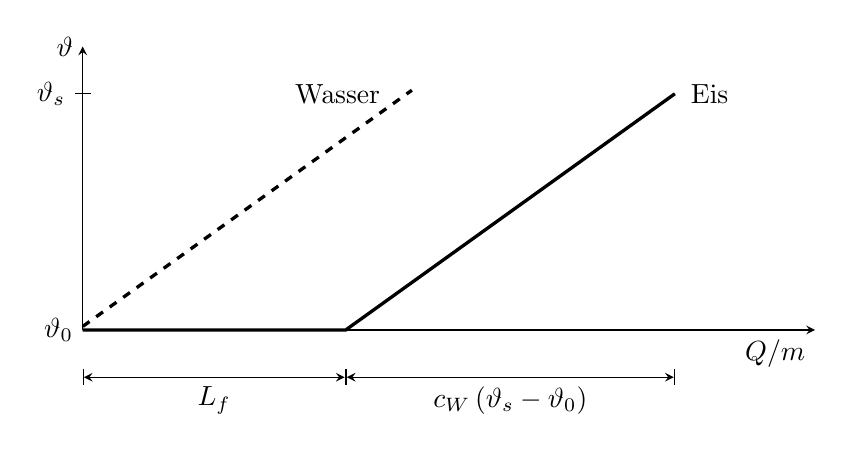
\begin{tikzpicture}[>=stealth, x=1cm, y=0.03cm]
 \draw[->] (0,0) -- (9.3,0) node[below left] {$Q/m$};
 \draw[->] (0,0) -- (0,120) node[left] {$\vartheta$};
 \draw (0.1,100) -- (-0.1,100) node[left] {$\vartheta_\text{s}$};
 \node[left] at (0,0) {$\vartheta_0$};
 \draw[very thick] (0,0) -- (3.34,0) -- (7.52,100);
 \draw[very thick, dashed] (0,1.5) -- (4.18,101.5);
 \draw[|<->|] (0,-20) -- (3.34,-20) node[midway, below] {$L_\text{f}$};
 \draw[|<->|] (3.34,-20) -- (7.52,-20) node[midway, below] {$c_\text{W}\left(\vartheta_\text{s}-\vartheta_0\right)$};
 \node[anchor=west] at (7.6,100) {Eis};
 \node[anchor=east] at (3.9,100) {Wasser};
\end{tikzpicture}
\end{center}

Das Wasser muss nur erwärmt werden, $Q_\text{W} = m\,c_\text{W}\left(\vartheta_\text{s}-\vartheta_0\right)$. Das Eis muss zuerst geschmolzen und dann gleich erwärmt werden, $Q_\text{E} = m\,L_\text{f} + m\,c_\text{W}\left(\vartheta_\text{s}-\vartheta_0\right)$. Beim Eis braucht es also zusätzlich $m\,L_\text{f}$, relativ zum Wasser
\begin{align}
 \frac{Q_\text{E}-Q_\text{W}}{Q_\text{W}} &= \mehrF \\
   &= \frac{\LfE}{\cW\cdot\left(\TsO-\TnO\right)} \\
   &= \mehr \approx \result{\mehrP{0}{2}}
\end{align}
mit $L_\text{f} = \LfEO$ (FoTaBe S.~190) und $c_\text{W} = \cWO$ (FoTaBe S.~191).
